\documentclass{sig-alternate}

\setcopyright{acmcopyright}
\conferenceinfo{GECCO'15 Companion,}{July 11--15, 2015, Madrid, Spain}
\isbn{978-1-4503-3488-4/15/07}\acmPrice{\$15.00}
\doi{http://dx.doi.org/10.1145/2739480.wk0907s}

\clubpenalty=10000
\widowpenalty = 10000
\usepackage[latin1]{inputenc}
\usepackage{amssymb}
\setcounter{tocdepth}{3}
\usepackage{graphicx}
\usepackage{subfigure}

\usepackage{url}

\begin{document}

\title{Designing and Modeling a Browser-Based Distributed Evolutionary Computation System} 

\numberofauthors{1}
\author{
\alignauthor 
J. J. Merelo Guerv�s and Pablo Garc�a-S�nchez\\
  \affaddr{GeNeura \url{http://geneura.wordpress.com}, Dept. of
    Computer Architecture and Technology \url{http://atc.ugr.es} and
    CITIC \url{http://citic.ugr.es}}\\ 
  \affaddr{University of Granada \url{http://www.ugr.university}}\\
  \email{(jmerelo,pablogarcia)@ugr.es}
}


\maketitle

\begin{abstract}
Web browsers have scaled from simple page-rendering engines to operating
systems that include most services the lower OS layer has, with the
added facility that applications can be run by just visiting a web
page. In this paper we will describe the front and back end of a
distributed evolutionary computation system that uses the browser's
capabilities of running programs written in JavaScript. We will focus on two
different aspects of volunteer computing: first, the
pragmatic: where to find those resources, which ones can be used, what
kind of support you have to give them; and then, the theoretical: how
evolutionary algorithms can be adapted to an environment in which nodes
come and go, have different computing capabilities and operate in
complete asynchrony of each other. We will examine the setup needed to
create a  simple distributed evolutionary algorithm using
JavaScript, with the intention of eventually  finding a model of how users react to it by
collecting data from several experiments featuring a classical
benchmark function. 
\end{abstract}

\keywords{Desktop grid, distributed computing, volunteer computing,
  Internet computing, socio-technical systems}

\section{Introduction}

The world has computational resources in spades, with every person
wielding one or more computational devices. The issue is how to make
them allocate even a small part of those resources to your particular
experiment. 

Most theory and experimentation in parallel computing has been devoted to predict and
optimize the performance in systems where the number of nodes, their
connections, and the time every one is dedicating to the computation is
known in advance as it often did in the Big Science era, where labs
could easily buy 16-node clusters or subscribe to the resources of a
big grid. Even today, you can rent instances of virtual machines in
the cloud relatively cheaply and use them for evolutionary computation
experiments \cite{sherry2012flex}. Nothing beats free, which is one of
the reasons why the era of
Citizen Science already started a few years ago (with SETI@home \cite{david-seti:home} and then BOINC \cite{boinc_grid04}) and it
offers a vast amount of computational resources to be used, if only
you know how to attract them. But there is a challenge: knowing, or at least having a
ballpark, of how your algorithm is going to perform in this uncertain
environment, where none of the factors is known: neither the number of
nodes, through how they are connected, to how long are they going to
be focused on doing what you want them to. That is why some effort is
needed to first understand the dynamics of the decision to participate
in an experiment that requires you to click on a link and then stay
for a while looking at the screen (or just leave it there
running). Volunteer computing experiments were set up for the first
time in the 90s, in the shape of the SETI@home screensaver
\cite{david-seti:home} that
analyzed signals looking for patterns indicating the existence of
extraterrestrial intelligence due to budget cuts by the US
congress. They proved \cite{anderson2006computational}
that 
\begin{quote}
... [V]olunteer computing can support
applications that are significantly more data-intensive,
or have high memory and storage requirements, than
those in current projects.
\end{quote}
Evolutionary algorithms are that kind of applications. In general,
real world problems and some combinatorial optimization problems such
as the MasterMind puzzle \cite{verbatim} do require an amount of
computational resources unavailable to the average researcher. On the
other hand, one clear advantage of volunteer computing frameworks is
its availability: in principle, any one can request volunteers. How
many she is able to gather, on the other hand, is an issue that we
will try to approach in this paper. 


Besides, since Amazon started selling EC2 several years ago, reliable
and scalable computing resources are also available for a low price
and on demand. Recently, Google has also refurbished its offering
lowering their prices. This means that the conjunction of free or
low-cost cloud computing engines, volunteer computing systems and
untapped capability of other people's desktop systems can be used for creating
massive, or at least potentially massive, distributed computing
experiments. These experiments can be easily set up using open-source
repository sites like GitHub\footnote{\url{http://www.github.com}} and deployed automatically to Platform as
a Service (PaaS) sites such as
Heroku\footnote{\url{https://www.heroku.com/}} or
OpenShift\footnote{\url{https://www.openshift.com/}} or even
Infrastructure as a Service (IaaS) sites such as Microsoft's Azure or
Amazon's EC2.


In general, it should be a requisite for volunteer computing
experiments  to be performed 
``in the open''. The fact that somebody is giving to you, basically for
free, computing resources, means that the scientist using them has to
give back; besides, people do not usually visit a resource unless they
can trust it; trust is an essential factor in the sharing of resources
such as this one, computing power \cite{van2009would}. The point of
departure for establishing this trust is releasing the source code used: all
volunteer computing platforms, from SETI@home on, have done it. The
opposite is probably the reason why many companies like PopularPower \cite{buyya2001compute}
have folded or others like CrowdProcess have decided to turn their
product to in-house computation \cite{ycombinator}: there must be a mutual relationship
of trust among the scientist and the person that is running his/her
code in the browser. As it has been mentioned in the early stages of what
was then called {\em desktop grid computing} \cite{gc:bausch}, in
fact CPU cycle selling might not make economic sense since there is
not so much demand for it and supply is quite high. However, while
potential supply is in fact huge, {\em actual} supply will depend on
the person holding it willing to actually allocate it to a particular
company selling it or a particular experiment needing it, not to
mention the fact that the experiment {\em actually} has to draw the
attention of the supplier, and thus it is better analyzed using the
Uses and Gratifications Theory \cite{severin2010communication}, that
is, taking into account {\em why} an user would do it, than using a
purely computational approach. That is why considering trust is
essential, and using free software might not be enough: Openness
has to progress from open source code to open science: releasing all
data obtained in the experiment in a repository such as GitHub,
mentioned above, and even allowing real-time access to experimental data
to users.

In fact, this relationship of trust is in many cases the only
mechanism preventing the malicious use of the system by creating bogus
solutions or simply attempting to exploit vulnerabilities by injecting
code. These problems have been analyzed in
\cite{Muszynski14vulnerabilities} but in principle our working
hypothesis will be that the clients using the browser are not
manipulating the code make the experiment finish before it should,
which is possibly the only way in which the experiment would be
affected. 

Another possible reason of the failure of former companies to create a
for-profit desktop grid might be the lack of a way to predict what is
going to be that supply in a particular moment. It is impossible to
predict, in advance, to know how many persons  are going to visit a
particular website. Even if you pull all the resources you have and
they lie across continents and time zones, the number of cycles
apportioned to a particular experiment will depend not only on the
users lending their web real state to the experiments (which is
usually the case for cycle brokerage companies) but especially to
users going to a web site and spending some time on them. Even if it
is theoretically impossible to predict to a high precision what
happens, it is in practice possible to approximate the number of
visits in a site, at least in a particular one, using time series. But
in the short term and looking at the big picture, there is still need
to model the behavior of users, so more factors can be added to
the model besides the time series of visits. This user behavior, of course,
presupposes that you are respecting their anonymity and privacy (not using
cookies, for instance) and that you are respecting the open science approach
mentioned above. All computation can be done without the knowledge of
the user \cite{unwitting-ec}, but this would work against openness
that would, curiously enough, result in a huge decrease of the future
performance of any experiment you might want to perform. 

These are best practices that have been followed in the experiments in
this paper, that first presents a new version of a platform for
distributed evolutionary algorithms (EAs) using the browser and a free (as
in free beer) backend, and second, shows the result from a
statistical point of view in order to put the basis for a model of the
meta-computer obtained by joining all volunteers and the free backend
used for the experiment. This has been one of the criterion when
choosing the different cloud services (hosting and logging, mainly):
the fact that they are free, and sustainably so
\cite{Merelo2014,jj:idc:lowcost}.
 
The work presented here is not intended to be an exhaustive or complete
exploration of the possibilities of this kind of volunteer and
distributed computation, but will allow us to describe, in general,
the behavior of the users 
as well as the performance achieved on the experiments done so far,
which should show some advantage over doing the same kind of
experiments locally using available resources. This performance will
be compared with other traditional island-based single user
client-server experiment using the same setup.

The rest of the paper is organized as follows: next we will present
the state of the art in volunteer computing and its modelling. We 
will proceed to describe the system and its experimental setup in Section
\ref{sec:exp}, some preliminary results in Section \ref{sec:res} and
finally we will present our conclusions in Section \ref{sec:conc}
along with future lines of work. 

\section{State of the art}
\label{sec:soa}

Using the web as a resource for distributed, or plainly user based,
evolutionary computation has a long history since JavaScript was
introduced as a browser-based language in 1997 and even before, when
other procedures, including Flash animations, VBScript, ActiveX or Java applets were
used. Java was pointed out in \cite{soares1998get} as a ``language for
internet'', providing some advantages such as multi-architecture compatibility or 
security mechanisms.
%\begin{quote}
%Java can bring some important advantages... solves architectural
%heterogeneity [...] easy to install and [...] built-in security
%mechanisms
%\end{quote} FERGU: quito esta cita y lo pongo sin el quote
% OK, pero �por? - JJ
In that work, Soares et al. describe JET, a system that supports
the execution of parallel applications over the Internet. This system has 
a comprehensive statistics support, allowing its use for science,
since it allows the collection of algorithm analytics by the
experiment designer, unlike the other systems compared in that paper.

However, Java (and all the other technologies)
is not universal in the
sense than an extra component, namely, the Java virtual machine, has
to be installed in the browser. JavaScript
\cite{flanagan2006javascript} was introduced in 1997 as a
browser-embedded language and has, since then, become a set of standards
\cite{ECMA-262} for the language, its components and future versions
that have been widely adopted by the industry and also by scientists,
who used them for creating a non-distributed EA on
the browser as early as 1998 \cite{jj-ppsn98}. 

The potential for volunteer computing using browsers was realized
later on \cite{sarmenta-bayanihan} as well as the potential for
mischief of users with code in their hands
\cite{sarmenta-sabotagetolerance}. However, these early efforts by
Sarmenta once again used Java and not JavaScript, making this effort
less universal. JavaScript can be used either for unwitting
\cite{unwitting-ec} or volunteer
\cite{langdon:2005:metas,gecco07:workshop:dcor} distributed
evolutionary computation and it has been used ever since by several
authors, including more recent efforts \cite{Desell:2008:AHG:1389095.1389273,duda2013distributed,DBLP:journals/corr/abs-0801-1210} that even
used the client's GPU \cite{duda2013gpu}. Many other researchers have
used Java \cite{chong:1999:jDGPi} and others have gone away from the
server-based paradigm to embrace peer to peer systems
\cite{jin2006constructing,10.1109/ICICSE.2008.99}. These computing
platforms avoid single points of failure (the server) but, since they
need a certain amount of infrastructure installed to start, the
threshold to join them is much lower. 

There have been relatively few efforts to analyze what is the
performance that can be obtained from these volunteer computing
effort. There was some attempt initially to dodge the issue by making
the algorithm adaptive to the kind of resources allotted to it
\cite{milani2004online}, which is actually not such a big problem in
algorithms such as the EA that can easily be
parallelized via population splitting or farming out evaluations to all
the nodes available. Lately, several approaches have focused on the
fault-tolerance of volunteer algorithms
\cite{gonzalez2010characterizing} which can, of course, be studied in
a more general distributed computing context
\cite{nogueras2015studying} or including it in a more general study of
performance of the EA itself %Con tu permiso lo paso a acrónimos para
                             %que no sea tan largo el párrafo. FERGU
%OK - JJ
\cite{DBLP:journals/gpem/LaredoBGVAGF14}. But the raw material of
volunteer computing, number of users and the time spent in the
computation in browser-based volunteer computing experiments, have only been studied in a limited way in
\cite{DBLP:journals/gpem/LaredoBGVAGF14} on the basis of a single
run. Studies using volunteer computing platforms such as SETI@home
\cite{javadi2009mining} found out that the Weibull, log-normal and Gamma distribution
modeled quite well the availability of resources in several clusters
of that framework; the shape of those distributions is a skewed bell
with more resources in the {\em low} areas than in the high areas:
there are many users that give a small amount of cycles, while there
are just a few that give many cycles. This is in concordance with the
results obtained in \cite{agajaj}.

As far as we know, this paper presents the only experiment that uses computational
resources that are as dissimilar as smartphones and powerful laptops
or desktop computers in a research center. The methodology used to
gather resources and the algorithms used will be described next, as
well as the results obtained with the setup.

\section{An island model in the browser}
\label{sec:exp}

% Rewrite this - JJ
In order to test the volunteer computing environment, a presentation
describing a low cost volunteer computing environment was
created. This presentation was actually delivered in several
conferences (such as IDC 2014, PPSN 2014 and FOSDEM 2015). These
results have been presented in \cite{arxiv:modeling}. In this paper,
although it uses exactly the same evolutionary algorithm client code,
the {\em presentation} has changed: it uses a single page with several
panels showing the progress of the algorithm and how many users have
been contributing to the experiment. To get users, the URL
(\url{http://nodio-jmerelo.rhcloud.com} and
\url{http://nodeo-i.herokuapp.com}) were presented, with a short
message, in Twitter and other social networks, introducing it as a
``demo for evolutionary algorithms'', sometimes in Spanish, some in
English. 

Besides visualizing the evolution, the browser is actually running an
distributed evolutionary algorithm that follows an  island model
\cite{muhlenbein1991parallel} using the server to transfer individuals from one browser to another in
what can be eventually a fully connected topology, although the term
does not correctly apply here.  

We will next explain the two framework tiers from the point of
view of the architecture itself and the algorithm that it is actually
running. First, we will describe the client code and next, in
subsection \ref{ss:server} the server architecture and where it is
hosted. 

\subsection{Volunteer distributed evolutionary computation in the
  browser}

As stated above, the evolutionary algorithms run mainly in the
browser. The problem run is a multimodal problem called {\em l-trap},
which has been used extensively as a benchmark for evolutionary
algorithms \cite{fernandes2009using,nijssen2003analysis}. This
function counts the number of bits in a sequence of $l$ and assigns
the local maximum if it has got 0 bits and the global maximum to $l$
bits. The fitness falls into a {\em trap} as you increase the number
of bits, that is why it creates a rugged fitness landscape that is
difficult to surmount for evolutionary algorithms. Its difficulty is
increased as the number of  concatenated traps grows, turning it into
a difficult problem for evolutionary algorithms. In
our case we have used $l=40$ traps. 

This fitness is implemented as part of the NodEO evolutionary
algorithm library written in node.js \cite{DBLP:conf/gecco/GuervosVGES14}, a server-based implementation of
JavaScript, converted to a client-based version via
``browserification''. The algorithm runs a Canonical evolutionary
algorithm on a population of 128, which is in fact too small for a
single node to find the solution; at least a population of 512 has
been found to be necessary to find the solution with a certain
probability. Initialization is random initialization and a canonical evolutionary algorithm
with an elite of 2 individuals is run, with crossover and then mutation applied
to all the population pool generated using 2-individual
tournament selection. The particular evolutionary
algorithm used is not so important, since we were rather focused on
the user behavior, although it is quite clear that the selective
pressure of the algorithm will have an impact in its performance and
will play for or against its asynchrony in many different and complex
ways \cite{jj:2008:PPSN}.

\subsection{Server side}
\label{ss:server} 

The server, that was also introduced during \cite{arxiv:modeling}, has
been rewritten in part to add new features that make experimentation
easier. I has been written using node.js and the {\tt express.js} and {\tt winston}
modules for REST and logging and includes the following REST \cite{Castillo12REST} 
routes:
\begin{itemize}
\item {\tt GET random} returns a random, non-evaluated individual,
  from the pool. The pool is just an array containing chromosomes,
  that is initialized at the beginning of the experiment.
\item {\tt PUT one} puts a single individual along with its fitness in the pool. In REST
  conventions, {\tt PUT} is used to create a resource, that is why it
  is used, in this case, to add a new individual to the pool.
\end{itemize}

These two routes are, in fact, an universal interface that can be
accessed from any program, written in any language that can connect
via HTTP.

The server program includes also additional logic for logging to
different files or services, routes to obtain information from the
server, such as the anonymized IPs that have participated in the
experiment, the ordinal number of the experiment that is being performed or the content of the chromosome pool, and code to serve the static pages
and the JavaScript/CSS
code also. 

The system described in this paper is fundamentally different from the
one published in 
\cite{arxiv:modeling}. This changes include, besides the inclusion of logging for a
better experiment analysis, the function that checks for the algorithm
termination condition and restarts the chromosome pool when
it does; it includes a configurable termination
condition that checks for the solution and empties the chromosome pool
and logs the end of the experiment. This allows us to run continuously
experiments without restarting the server by hand as we did in the
previous version. The evolutionary algorithm itself has not changed,
but the facilities for modelling user behavior have improved, as shown
later on in the paper. 

In this experiment we have used OpenShift (\url{http://openshift.com})
and Heroku (\url{http://heroku.com}) which are Platform as a Service products with a
free tier. It could be also be deployed, with small
or no modification, to other similar PaaS such as BlueMix by IBM,
maybe with a bit of adaptation. Any of them are
free up to a certain level of use and thus fulfill the requirement of
using free resources as a sustainable way of performing distributed
evolutionary computation experiments \cite{Merelo2014,jj:idc:lowcost}.
%
\begin{figure*}[h!tb]
        \centering
        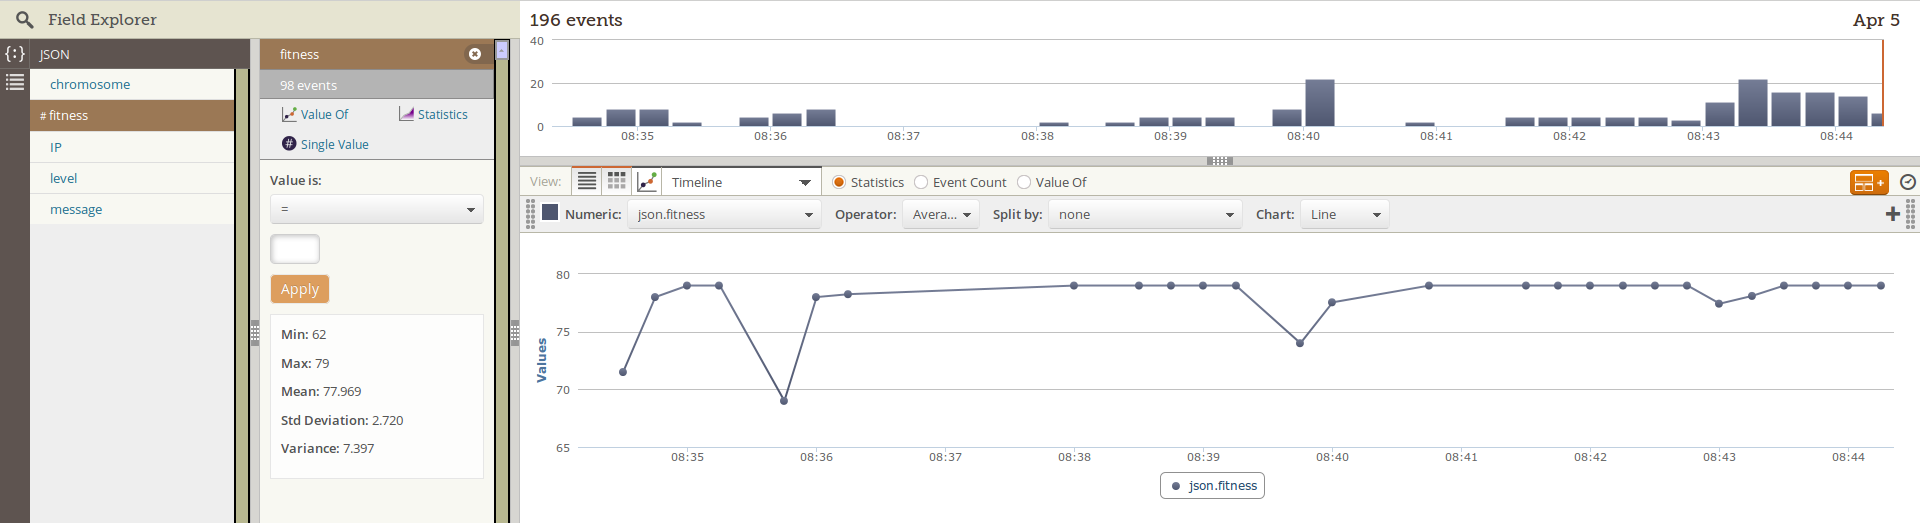
\includegraphics[width=0.9\linewidth]{img/loggly.png}
        \caption{Loggly dashboard showing the evolution of fitness for
        the last 10 minutes of an experiment.}\label{fig:loggly}
\end{figure*}

Programming the server so that it can be deployed, without
modification, to any PaaS, does not add a lot of overhead to the
programming of a framework, but you have to consider
the different capabilities of each one, namely:\begin{itemize}
\item Heroku does not have a permanent filesystem, so if you want to
  create any directory it has to be done when the server is
  started, and it is only guaranteed to last while the application is
  running; this also implies the need for an external logging system
  to keep the results.
\item In order to scale properly, all requests in Openshift are routed
  through a proxy. This means that all requests have, as remote
  address, the proxy's IP, so other ways of obtaining the requests must be found
  out. On the other hand, it does have a permanent directory for
  data. 
\end{itemize}

Every PaaS has its own way of defining environment variables, which is
the mechanism 
used for passing private configuration information such as database
passwords or, in our case, logging system keys, to the
server. This can be done usually through a command-line client ({\tt
  heroku} or {\tt rhc}), which is also used to check the logs or
restart the client. Eventually, we decided to leave the two servers
running. 

Having the pages and the server in the same domain allows to work in the
default Ajax mode, that does not allow cross-site requests, that is,
requests from a page to a domain different from the one it has been
served. However, 
%FERGU: no todo el mundo sabe de Ajax y lo de cross-site, expl�calo
%mejor
%explicado - JJ
these can also be enabled if needed so that the static pages and the
REST server can be hosted in different servers, allowing the genetic
algorithm code to {\em parasite} other pages. 

In this framework every server holds %FERGU: si es referencia a lo de
                                %parasitar de arriba ponlo en el mismo
                                %p�rrafo, que parece que te refieres a
                                %lo "parasitar". Mejor "In this
                                %study"? 
% No, se refiere a que no es un sistema multi-experimento - JJ 
a single experiment, there is no multi-tenancy of experiments, so its
management is quite simple. A different experiment would need to
deploy and start a server that serves different code and checks for
different termination conditions.


During and after the experiment, the data can be collected from one of
the logs: the server log file, data files (that cannot be used in
Heroku, for instance)  or from online logging services such as
Loggly (\url{http://loggly.com}), which is the one we are using. Loggly was chosen for its
easiness and support from the {\tt winston} logging library as well as
its graphing capabilities, shown in Figure \ref{fig:loggly}; however,
it is only free for a month, so a more sustainable alternative (read:
free and open source) will have to be sought in the future, after this paper is finished. Other online logging %FERGU: esto de que "despues de que se termine el paper" no me mola mucho.
services have a free tier that can be used forever; however, its
support and graphing facilities were not so complete. Choosing a good logging
service for experiments in open science is, for us, an open issue, and it is
outside the scope of this paper, so it will have to be left for future
work.


As indicated in the introduction, every part of the experiment and
data gathered have been released as free software in the GitHub
repository \url{https://git.io/nodio}, and they 
will be analyzed in the next section.

\section{Results}
\label{sec:res}

The experiments done with the first versions of this framework have
already been published elsewhere \cite{arxiv:modeling}. We proved that
up to 20 nodes could participate in a single run if it was
sufficiently announced; every experiment was individually announced so
more or less a certain amount of nodes were guaranteed. However, it
did not run correctly in mobile phones, design of the presentation was
not adaptive and thus missed a good amount of possible clients. In
this case the design, which has used the Kube CSS framework, was fully
adaptive and indeed proved to work with mobile phones browsers for
iPhones and Android phones. 
%
\begin{figure}[h!tb]
  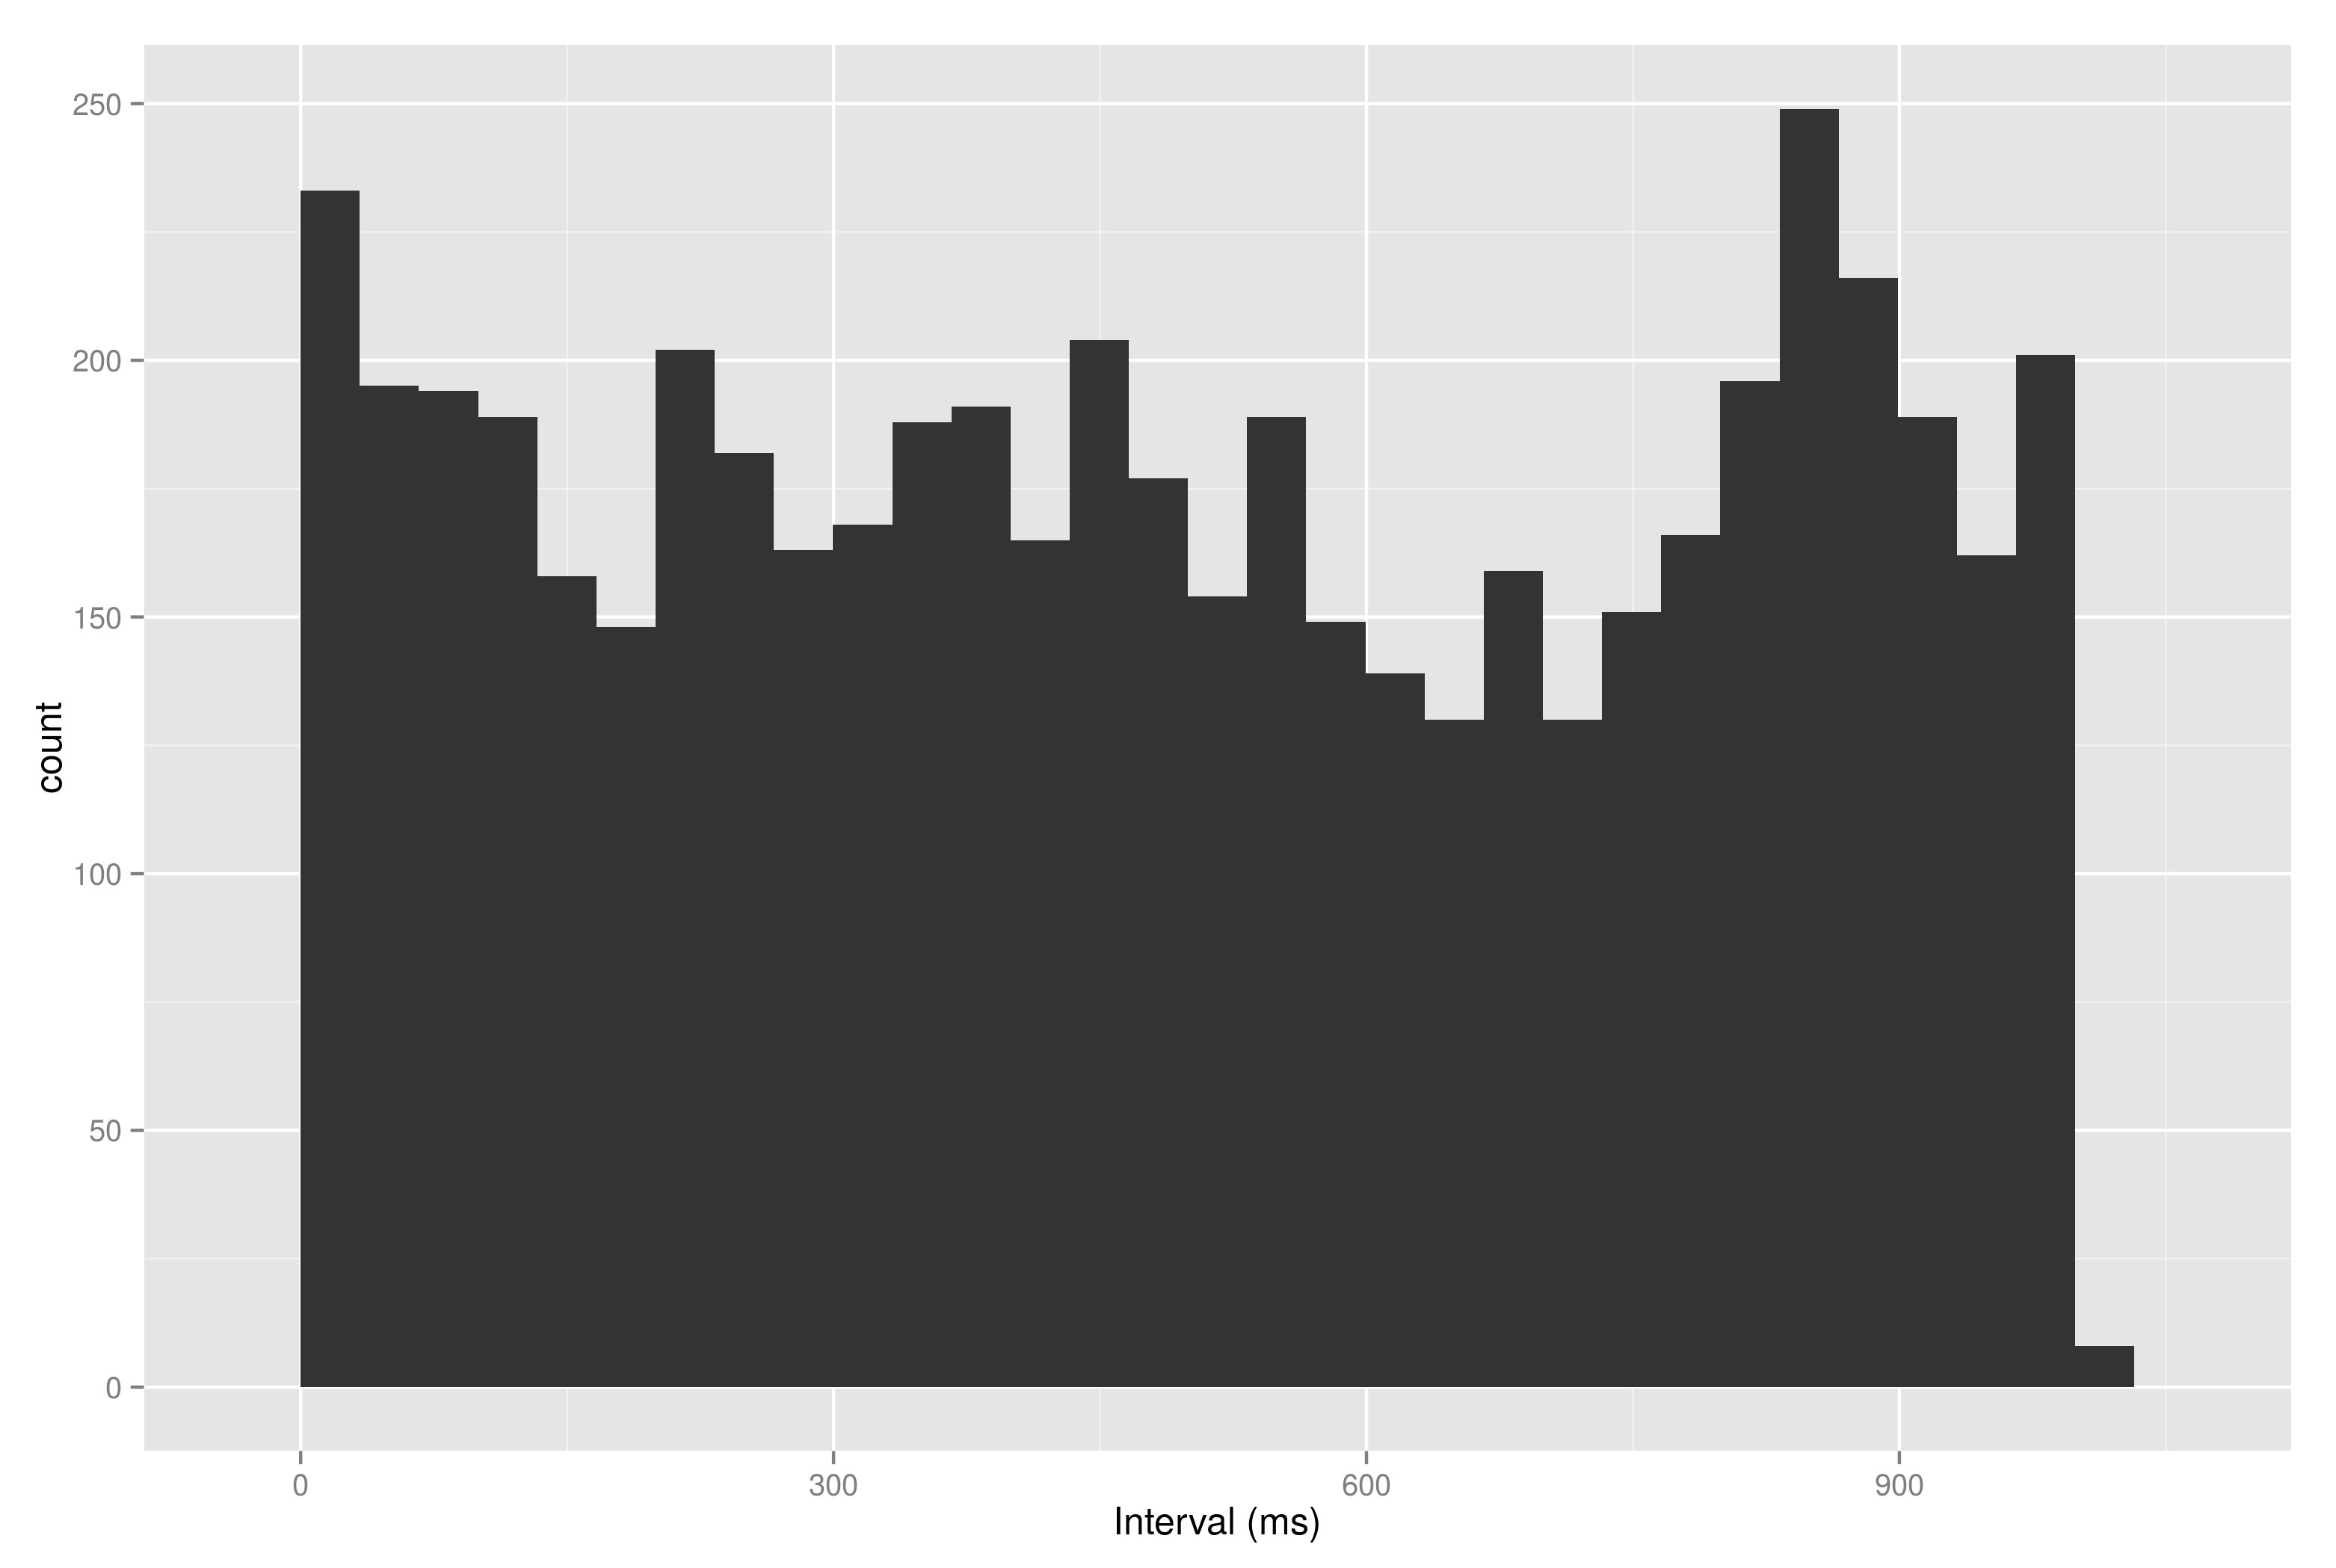
\includegraphics[width=0.95\linewidth]{img/openshift-intervals.png}
  \caption{Histogram of the intervals between two requests by the same
  IP for all experiments in the OpenShift server.}  \label{fig:intervals}
\end{figure}
%
\begin{figure*}[h!tb]
  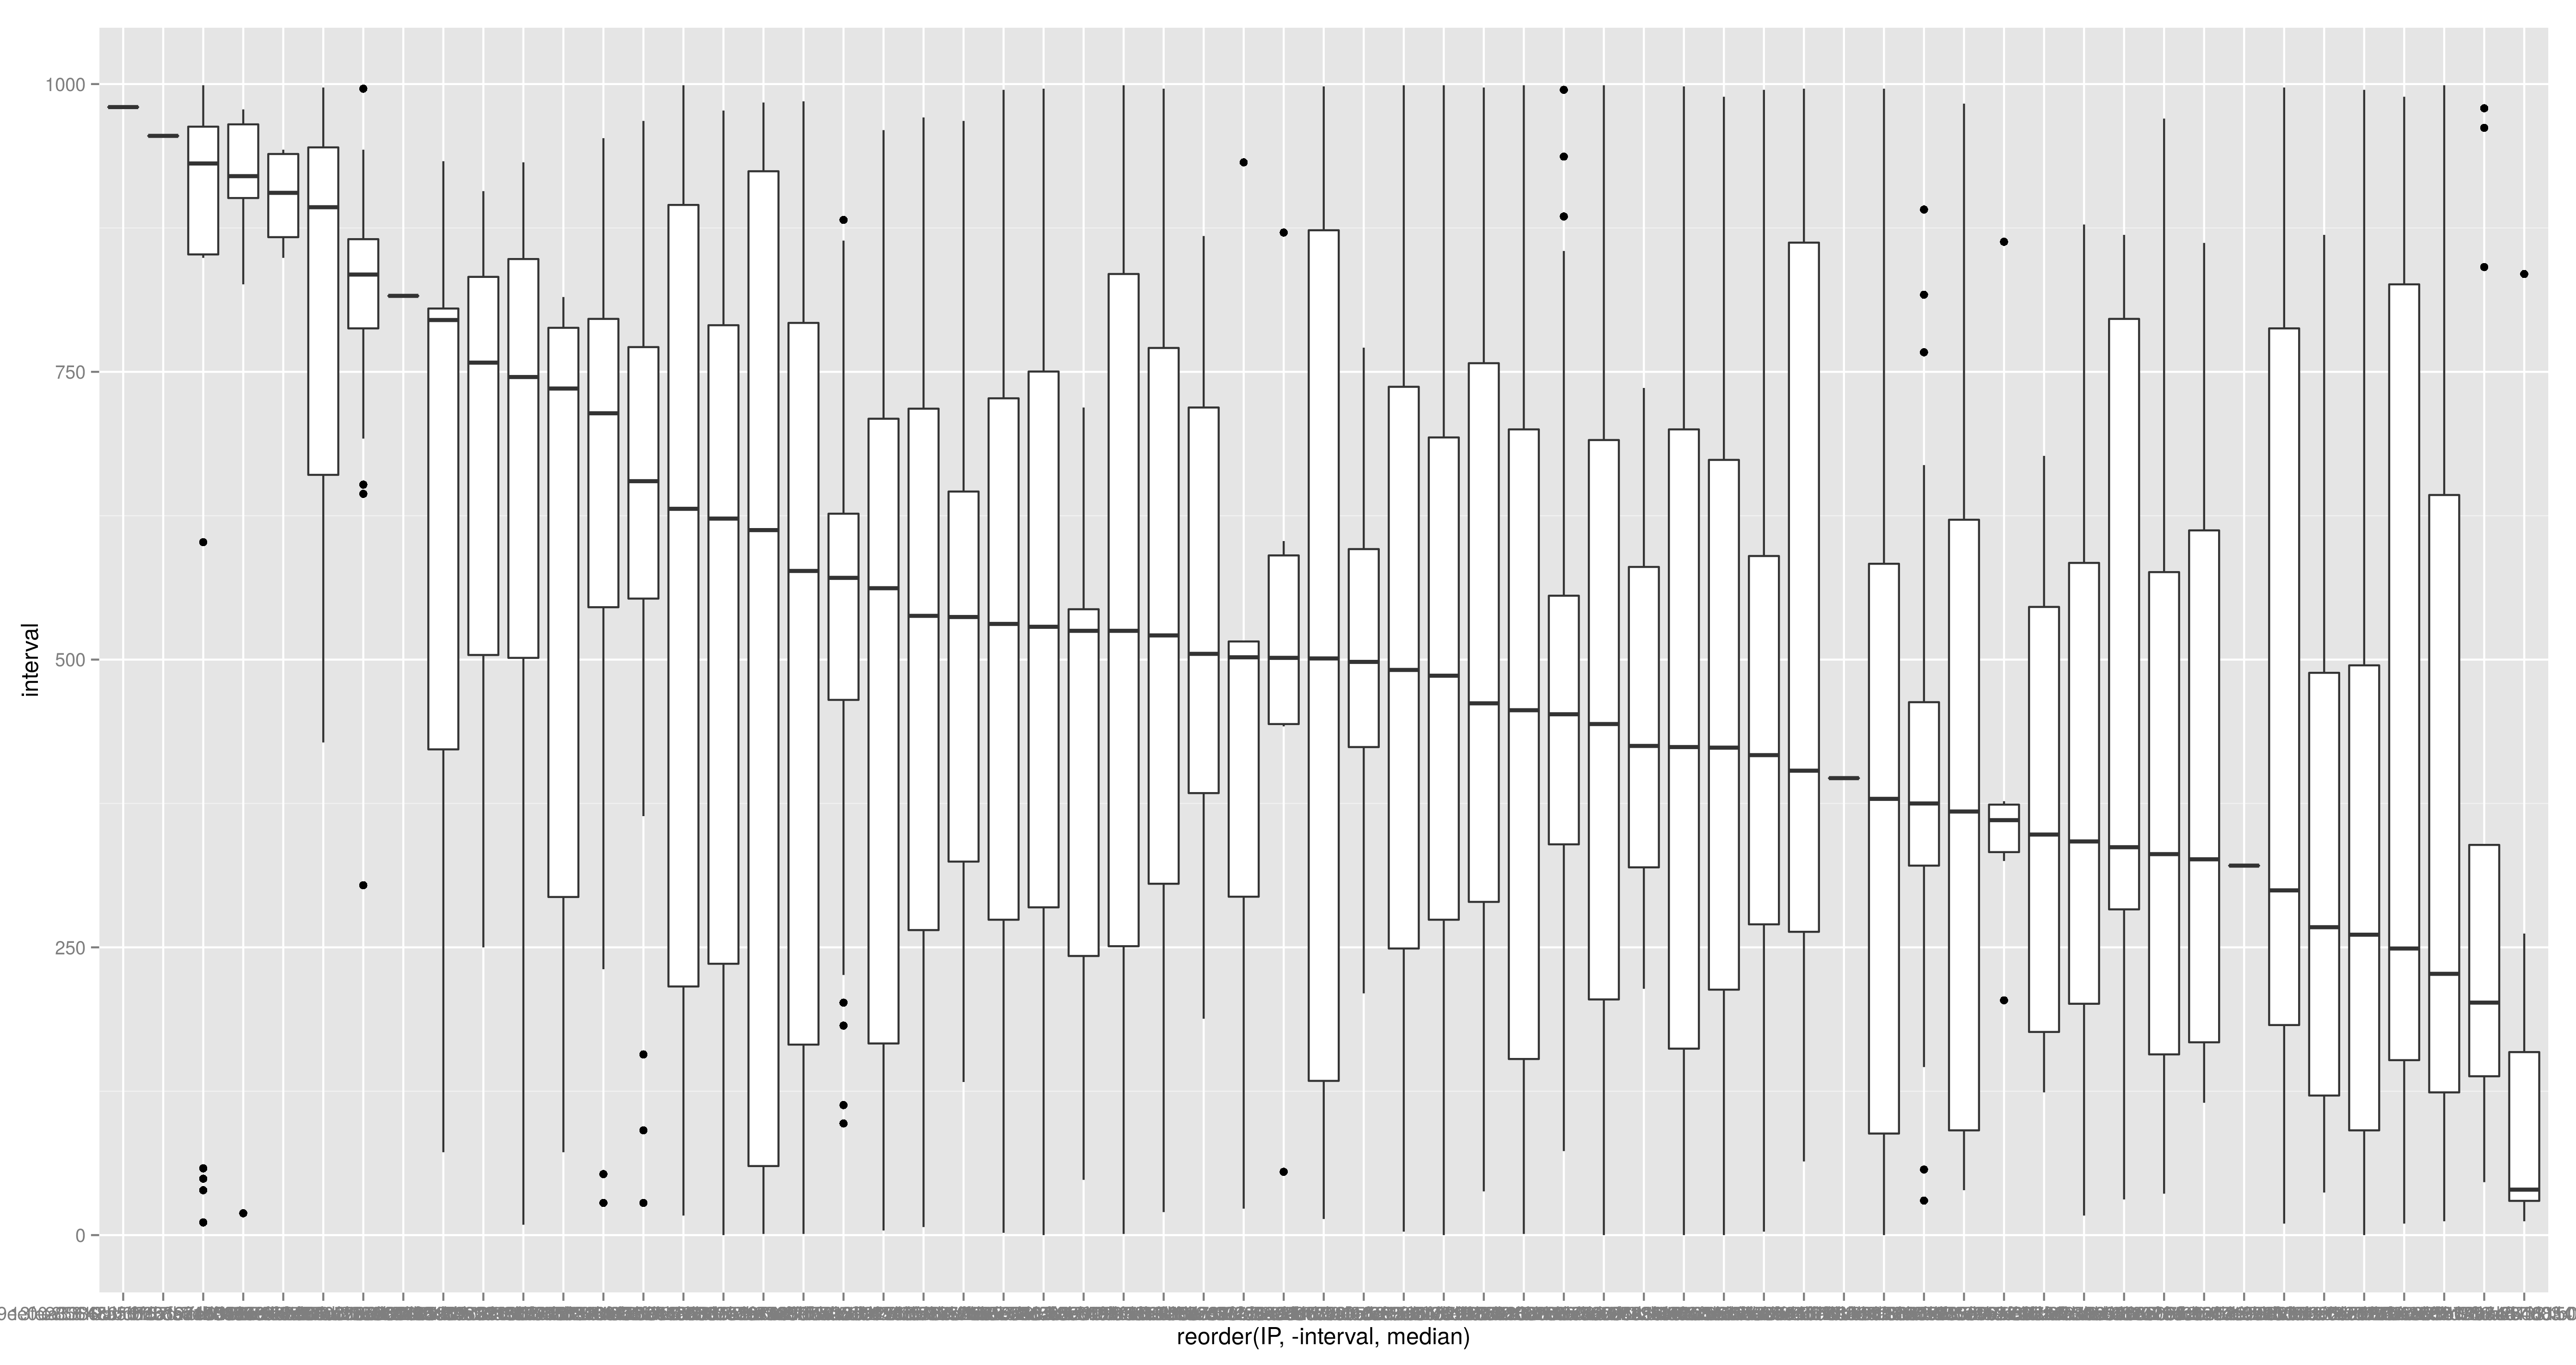
\includegraphics[width=0.90\linewidth]{img/openshift-intervals-IP.png}
  \caption{Boxplot of the intervals between two requests by the same
  IP, by IP, ordered by descending median.}  \label{fig:intervalIP}
\end{figure*}

At the time of this writing, 23 runs were done in OpenShift and one in  
% para trabajos futuros, estas cifras de cu�ntas ejecuciones se han completado 
% quiz�s habr�a que presentarlas de forma diferente. Quiz�s indicando el tiempo
% total de "puesta online" del sistema, c�mo se publicit� para atraer gente,
% y entonces ah� contar las estad�sticas de cu�nta gente partici�, cu�ntas
% ejecuciones se terminaron, etc.  [Pedro]
% se terminaron todas. Lo de cuanta gente por ejecuci�n (cuantas IPs,
% en realidad) y cuanto tardaron no lo he llegado a analizar, aunque
% tengo los datos. Se deja para trabajo futuro, puedes a�adirlo a un
% issue - JJ
Heroku. The Openshift URL was mentioned more frequently than the other
so that accounts for the popularity, not any particular problem with
the algorithm in one or the other. That is why the data that we have
obtained and used below, and which is, as usual, available with a free
license, is mainly processed from the log files stored in Loggly and
in OpenShift. These 23 experiments took each one a number of hours, so
that in many cases the nodes were not accessing at the same time, but
sequentially, to the server. This means that the island model is, in
fact, behaving partly as a pool-based evolutionary algorithm
\cite{sofea:evopar2012} with some results, the best from each
generation, available to future runs. This is clearly noticed when
visualizing the algorithm: its behavior changes when it gets its first
chromosome from the pool, in many cases improving a lot.

However, due to the small population we are using, this sometimes
means stagnation and a long time to run so the first lesson we have
learned here is that adaptation of at least the population size to the
distributed, pool-based and asynchronous setup should be studied more
carefully and probably use a randomized parameter setting as we did in
\cite{sofea:evopar2012}. 

Another interesting result is that we have been able to obtain many
more different users. At the time of this writing we obtained 75
different IPs contributing CPU time to the experiment, giving an
% �se podr�a hacer en el futuro alg�n tipo de estudio acerca de la procedencia?
% No estoy seguro de que esa relevante, pero bueno...   [Pedro]
% �Por pa�s? Por referrer igual s�... Tambi�n a��delo como issue - JJ
average of around 4 per experiment. However, there is a big variation
in the number of CPUs. There is also a much bigger range in the
performance of these clients. In order to measure that we have
computed the time between two requests from the same IP and plotted it
as an histogram in Figure \ref{fig:intervals}. In that histogram we
can see that there is an almost uniform distribution of intervals,
from the smallest taking a few milliseconds to the biggest with almost
1 second; the setup of the experiment allows it to be accessible from
a very wide range of different IPs. Even within a single IP the
variation can be relatively high, which is shown in a boxplot in
Figure \ref{fig:intervalIP}, sorted by median time. The time between
requests to the server, that is, the time to process 100 generations
of 128 individuals of an evolutionary algorithm to optimize the Trap
function has also very wide range, but even within the same IP,
inter-quartile differences of several hundred milliseconds are not
uncommon. Median for all IPs is 485 milliseconds and average is quite
close, at 496.8 ms. 

Some interesting conclusions can be drawn from this data. The first is
not new: we need frameworks able to work with asynchronous algorithms
to take advantage of all the processing power that is available in an
ad-hoc, ephemeral, setup such as the one available in evolutionary
algorithms. The second is that there is going to be CPU available from
volunteers even when no active announcement is made, just from people
that come from a link in a social media page or the Twitter
timeline. However, an announcement brings immediate attention to the
page which will, obviously, depend on the popularity of the social
media and the person announcing it. How this dependency behaves is
still an open issue. Finally it is also an interesting conclusion
that, given enough time and free computing power, we can solve a
difficult optimization problem. Eventually. But for free.


\section{Conclusions}
\label{sec:conc}

In this paper we have presented our experience on using browser-based
computing applied to the design of evolutionary algorithms and an
analysis of user behavior focused on the type of device, represented
by its performance, they will be using to access the URL that holds
the experiment. In the
spirit of Open Science, we have released all material related to the
experiment, including this paper. Experiments have been performed at
several times of the day and announced in Twitter, LinkedIn  or other
social media. 

From the last experiment published we concluded that the nature of the
performance, which is due to the number of persons deciding to
participate in the experiment, is not totally random. There are at
least lower bounds we can count on: several computers (as few as six)
can almost always be relied on, and in some cases up to 30 can
participate in a single experiment. However, it is not clear how all
these computers contribute to the overall performance in terms of
time, although all experiments were performed until a solution was
found. In the last experiment, performed mainly in front of a live
audience using laptop computers, most of the participants in the experiment were in the same
performance tier, although a small percentage of them (which will be
around 25\%) are quite slow. In this experiment the conclusion is
different: uniform distribution of performance from quite slow to
blazing fast, with approximately 50\% slower than the average and,
conversely, 50\% faster. Our algorithm should, then, cater to a very
wide performance range so some methodology for self-adaptation should
be used on the evolutionary algorithm running in the browser. A more
precise model of the user is needed also in order to properly design
the algorithm, carrying it further away from the canonical
evolutionary algorithm we are using right now, which can only take
performance so far. 

More
systematic experimentation is also needed, specially using different
kind of problems, including more complex ones in which the fitness
function is {\em heavier} and takes longer to be processed. However,
the main intention of this paper, which was to provide some initial
measures on how the users of an volunteer evolutionary algorithm
experiment would behave, has been reached. 

There are many issues involved in using these resources: from adapting
current algorithms so that they match this environment 
to check which EA configuration works the best in it, or creating a
framework that can use it easily. But the main
challenge is that asking people to contribute resources implies that
you are opening your science to society and you have to give something
in return: you have to adopt a set of best practices that have come to
be known as Open Science, because ``Give, and it shall be given unto
you'', you will get as much back from society as you give to it
opening your science and explaining it to the public. In this paper,
we have shown some algorithmic visualization so that at least it is
visually attractive; in the previous experiment it is a
presentation. But there are many other possible ways of doing it,
including measuring the effect of a stealth algorithm which does not
shown anything at all. Some intriguing effects on how the experiment
is announced have also been noticed. While an announcement in English
attracted no new user, another in Spanish did attract immediately
several of them. Due to the popularity of WhatsApp groups, we would
like to test what happens with them, and how many will be visiting the
URL as a percentage of the users compared with the usage rate of
Twitter or Facebook.

It also remains to be done a comparison of single-desktop computer
experiment compared with this parallel setup. It is quite clear that,
due to overhead, several volunteers will be needed to match the speed
of a single multicore desktop computer. This will be explored in
future work.

\section{Acknowledgments}

This work has been supported in part by TIN2011-28627-C04-02 and
TIN2014-56494-C4-3-P (Spanish Ministry of Economy and Competitivity),
SPIP2014-01437 (Direcci{\'o}n General de Tr{\'a}fico) and PYR-2014-17
GENIL project (CEI-BIOTIC Granada). We would also like to thank the
anonymous reviewers of this paper who have really helped us to improve
this paper (and our work) with their suggestions.

\bibliographystyle{abbrv}
\bibliography{geneura-latin1,volunteer,javascript,ror-js,GA-general}

\end{document}
%%% Local Variables:
%%% ispell-local-dictionary: "english"
%%% End: